\begin{quest}[Stelling van Rice]
	Leg de stelling van Rice uit en geef het bewijs. Geef minstens \'e\'en eigenschap van Turingmachines die niet voldoet aan de voorwaarde voor de stelling van Rice en toon aan dat die eigenschap geen aanleiding geeft tot een niet-beslisbare taal. Karakteriseer volledig alle eigenschappen van Turingmachines die aan de stelling van Rice voldoen m.b.v. $IsIn_{TM,S}$.
\end{quest}

\subsubsection*{De stelling van Rice}

Vooraleer we verder gaan met de stelling van Rice is het verstandig om sommige termen te verklaren. Niet-triviale en taal-invariante eigenschappen zijn een belangrijk onderdeel van de stelling. In onderstaande verklaringen duidt $Pos_P$ op de verzameling van machines die in het bezit zijn van een eigenschap $P$ en $Neg_P$ de verzameling van machines zonder eigenschap $P$.

\begin{theorem}[Niet-triviale eigenschap]
	Een eigenschap $P$ van Turingmachines heet niet-triviaal indien $Pos_p \neq \emptyset$ en ook $Neg_p \neq \emptyset$. Er bestaan dus Turingmachines die deze eigenschap $P$ bezitten, maar ook machines die deze niet bezitten.
\end{theorem}

\begin{theorem} [Taal-invariante eigenschap]
	De eigenschap $P$ heet taal-invariant indien alle machines die dezelfde taal bepalen hebben ofwel allemaal $P$, ofwel heeft geen enkele ervan $P$.
	$$L_{M_1} = L_{M_2} \Rightarrow P(M_1) = P(M_2)$$
\end{theorem}

\noindent Met deze twee definities in het achterhoofd, kunnen we overgaan naar de formele definitie van de stelling van Rice, met het bewijs als gevolg.

\begin{theorem}[Stelling van Rice]
	Voor elke niet-triviale, taal-invariante eigenschap $P$ van Turingmachines geldt dat $Pos_P$ (en ook $Neg_P$) niet beslisbaar is.
\end{theorem}

\begin{proof}
	We bewijzen dit met behulp van een contradictie. Neem de Turingmachine $M_\emptyset$ die de lege taal beslist. Laten we er nu van uit gaan dat deze machine een bepaalde eigenschap $P$ heeft. De stelling zegt ons dat de eigenschap $P$ niet-triviaal en taal-invariant is. Uit de definitie kunnen we dan afleiden dat $Pos_P \neq \emptyset$ (en ook $Neg_P \neq \emptyset$). Aangezien deze verzameling niet leeg is, moet er een Turingmachine $X$ bestaan met deze eigenschap $P$. Laat ons zeggen dat deze Turingmachine de taal $L_X$ beslist.\\\\
	We gaan nu proberen een contradictie te bekomen door aan te nemen dat de stelling niet waar is. We nemen dus aan dat $Pos_P$ (en dus ook $Neg_P$) beslisbaar is. We gaan nu een beslisser $B$ proberen op te stellen voor $Pos_P$ die deze beslist\footnote{Later zullen we deze $B$ gebruiken om een beslisser $A$ te maken voor de taal met Turingmachines $A_{TM}$}. Om $B$ te maken, gaan we eerst een hulpmachine $H_{M,s}$ opstellen.\\\\
	Deze hulpmachine $H_{M,s}$ heeft een Turingmachine $M$ en een string $s$ in zich. Deze staan vast voor de machine en kunnen dus niet veranderen\footnote{Ze zijn als het ware gehardcoded.}. De input van deze machine is een string $x \in L_X$. Wanneer $H_{M,s}$ gestart wordt, zal deze eerst $M$ laten lopen over $s$. Indien $M$ $s$ reject, zal $H_{M,x}$ altijd rejecten. Indien $M$ $s$ accept, dan zal $H_{M,s}$ overgaan naar fase 2. Hier zal de hulpmachine $X$ over $x$ laten lopen. Indien $X$ $x$ ook accept, dan zal de hulpmachine accepten. Indien $X$ $x$ reject, dan zal ook de hulpmachine rejecten.
	\begin{figure}[H]
  	\centering
    	  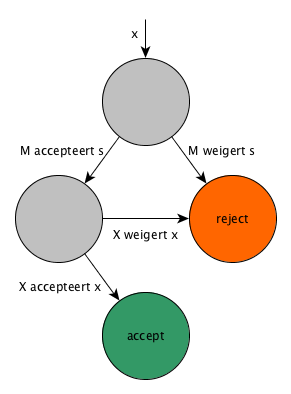
\includegraphics[width=0.3\textwidth]{./img/HMs}
  	\caption{Concept van $H_{M,s}$}
	\end{figure}
	Er zijn nu twee mogelijkheden voor $H_{M,s}$. Indien $M$ $s$ accept, dan gaat $H_{M,s}$ altijd overgaan tot het testen van $x$ in $X$. In dit geval beslist $H_{M,s}$ de volledige taal $L_X$. De andere optie is dat $M$ $s$ reject. In dat geval gaat de hulpmachine altijd rejecten en dus enkel de lege taal accepteren.\\\
	Laat nu de beslisser $B$ los op $H_{M,s}$. Dit wil zeggen dat de beslisser accept of reject voor de gegeven $M$ en $s$.\\
	Stel dat we nu een beslisser $A$ maken voor $A_{TM}$. In dat geval moeten we dus elke $M$ en $s$ in $A_{TM}$ testen. We kunnen dus zeggen dat $A$ accept indien $B$ $H_{M,s}$ accept, anders reject. We bekomen dus de volgende conclusie.
	\begin{center}
		$A$ accepts $<M,s>$\\
		$\Updownarrow$\\
		$B$ accepts $H_{M,s}$\\
		$\Updownarrow$\\
		$H_{M,s}$ heeft eigenschap $P$\\
		$\Updownarrow$\\
		$H_{M,s}$ accepts $L_X$\\
		$\Updownarrow$\\
		$M$ accepts $s$
	\end{center}
	Conclusie: $A$ is een beslisser voor $A_{TM}$, maar dit is onmogelijk aangezien $A_{TM}$ niet beslisbaar is\footnote{Zie vraag 1 van dit hoofdstuk voor het bewijs.}. Hieruit kunnen we concluderen dat alle bovenstaand equivalenties onwaar zijn en dus is  ook $Pos_P$ niet beslisbaar. Contradictie.
\end{proof}

\subsubsection*{Voorbeeld}

We nemen de Turingmachine $TM$ als voorbeeld. We stellen ons de vraag over de volgende eigenschap. Zal de Turingmachine $TM$ ooit zijn leeskop naar links verschuiven? We kunnen hier een beslisser voor opstellen.
\\\\
Gegeven het tupel $<M,s>$ zal $TM$ $M$ loslaten op $s$ voor maximaal $|s|$ stappen. Als de machine geen enkele keer zijn leeskop naar links heeft bewogen, dan moet de leeskop op de eerste $\#$ staan aan de rechterkant achter $w$ op de leesband. Zoek nu de overgang $\delta$ in het state diagram van $M$ die $\#$ als input heeft. We zijn enkel ge\"intereseerd in deze, aangezien voor de andere de leeskop nooit naar links is gegaan. Indien geen enkel van deze transacties naar links gaat, accept. Indien een van hun wel naar links gaat, reject.

\subsubsection*{Algemene notatie}

De volgende notatie bepaalt de verzameling van turingmachines $M$ die een taal $L_M$ bepalen die behoren tot een gegeven verzameling van talen $S$.
$$IsIn_{TM,S}=\{<M,S>|L_M \in S\}$$
We kunnen deze notatie gebruiken om eigenschappen te karakteriseren. Een voorbeeld van een eigenschap van $E_{TM}$ die voldoet aan de voorwaarden van de stelling van Rice, is dat de bepaalde taal leeg is. We kunnen dan de volgende notatie gebruiken om de eigenschap te karakteriseren.
$$E_{TM} = IsIn_{TM,\{\phi\}}$$
